\documentclass[12pt,a4paper]{scrartcl}

\usepackage[ngerman]{babel}
\usepackage[ansinew]{inputenc}

\usepackage{float}

\usepackage[pdftex]{graphicx}
\usepackage{latexsym}
\usepackage{amsmath,amssymb,amsthm}
\usepackage[linesnumbered,ruled]{algorithm2e}
\usepackage[table]{xcolor}
\usepackage{subfig}
\usepackage{listingsutf8}

\lstset{ % General setup for the package
	language=Java,
	basicstyle=\small\sffamily,
	numbers=left,
	numberstyle=\tiny,
	frame=tb,
	tabsize=2,
	columns=fixed,
	showstringspaces=false,
	showtabs=false,
	keepspaces,
	commentstyle=\color{red},
	keywordstyle=\color{blue}
}

% Abstand obere Blattkante zur Kopfzeile ist 2.54cm - 15mm
\setlength{\topmargin}{-15mm}


\begin{document}
	
	% Keine Seitenzahlen im Vorspann
	\pagestyle{empty}
	% Titelblatt der Arbeit
	\begin{titlepage}
		
		\begin{center}
			\vspace*{2cm} 
		\end{center}
		
		\begin{center} \large 
			
			Praxisprojekt
			\vspace*{1cm}
			
			{\huge Half-Edge Mesh f\"ur Unity3D}
			\vspace*{1.5cm}
			
			Erstellt von:\\
			Yannick Dittmar\\Studiengang: Allgemeine Informatik\\ Matrikelnummer: 11117676
			
			\vspace*{1.5cm}
			
			Datum der Abgabe: xx.xx.xxxx
			\vspace*{1.5cm}
			
			Betreuung: Dennis Buderus \\[1cm]
			Technische Hochschule K\"oln\\
			Fakult\"at f\"ur Informatik und Ingenieurswissenschaften
		\end{center}
	\end{titlepage}

\tableofcontents

\pagestyle{headings}

\section{Abstract}
Das Ziel dieser Arbeit ist es, die Performance von Unity-Meshs mit der eines Half-Edge Mesh zu vergleichen. In dieser Arbeit wird versucht, die folgende Forschungsfrage zu beantworten: Wie unterscheidet sich die Laufzeit von Unity-Meshs und Half-Edge Meshs, bei der Ausf\"uhrung von Standartmethoden f\"ur dynamische Anwendungen und was bedeutet dies f\"ur ihre Anwendungsbereiche?
Um diese Frage zu beantworten, wird ein Prototyp entwickelt und das Half-Edge Mesh theoretisch betrachtet, um Aussagen \"uber das durchschnittliche Laufzeitverhalten treffen zu k\"onnen.
Diese Analysen haben gezeigt, dass sich Half-Edge Meshs durch ihre deutlich bessere Laufzeit f\"ur dynamische Meshs besser eignen, daf\"ur allerdings einen h\"oheren Speicherbedarf aufweisen. Deshalb sollte bei gr\"o{\ss}eren Meshs abgewogen werden, ob der Anwendungsfall ein Half-Edge Mesh ben\"otigt oder ob die native Unity-L\"osung ausreichend ist.
\section{Grundlagen}
Dieses Kapitel besch\"aftigt sich mit den Grundlagen, die f\"ur diese Arbeit relevant sind. Dabei geht es sowohl um die Entwicklungsumgebung Unity3D, als auch um das Konzept der Triangluar Meshes, die essenziell in der 3D-Computergrafik sind.

\subsection{Unity3D}
Unity3D ist eine plattform\"ubergreifende Spiele-Engine mit eingebauter Entwicklungsumgebung f\"ur zwei- und dreidimensionale, sowie Augmented- und Virtual-Reality Spiele und Simulationen. Die Engine besitzt einen eigenen Editor, in dem diverse Szenarien erstellt und bearbeitet werden k\"onnen. Um diese Szenarien zum Leben zu bringen unterst\"utzt Unity selbst programmierte Scripte auf der Grundlage von C\#. Insgesamt laufen auf \"uber drei Milliarden Ger\"aten Programme, die mit Unity erstellt wurden, auf \"uber 25 verschiedenen Plattformen, wie Windows oder Linux und den g\"angigen Spielekonsolen wie die PlayStation 4, XBox One und der Nintendo Switch. Zudem sind 50\% aller mobilen Spiele und 60\% aller VR/AR Anwendungen mithilfe von Unity entstanden \cite{Unity}. Spiele wie ,,Pok\'emon Go'', ,,Superhot'' und das Simulationsspiel ,,Universe Sandbox'' sind drei Beispiele f\"ur Spiele, die in Unity erstellt wurden.

\subsection{Triangular Meshes}
Um auf einem Computer eine dreidimensionale Szene, zum Beispiel mit der Hilfe von Unity darzustellen, m\"ussen alle dargestellten Modelle angen\"ahert werden. In der Regel werden daf\"ur Dreiecksnetze (Triangular Mesh) verwendet, die die Oberfl\"ache eines Objekts mithilfe von Dreiecken ann\"ahert, wie in Abbildung \ref{fig:dolphintrianglemesh} anhand eines Delfins gezeigt. Informationen, die f\"ur ein solches Dreiecksnetz garantiert ben\"otigt werden, sind eine Reihe von Eckpunkten, den Vertices, die immer in Dreiermengen kommen und deren Position im dreidimensionalen Raum \cite[S.262]{Shirley2010}. Diese werden durch Kanten (Edges) verbunden und bilden damit Dreiecksfl\"achen, auch Faces genannt.

\begin{figure}[h]
	\centering
	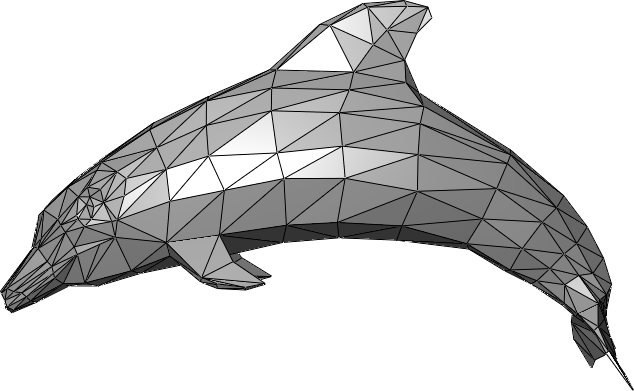
\includegraphics[width=0.7\linewidth]{Images/Dolphin_triangle_mesh}
	\caption[Beispiel eines Polygonen-Netzes]{Beispiel eines Dreiecks-Polygonen-Netz, von \cite{WikipediaDolphin1}}
	\label{fig:dolphintrianglemesh}
\end{figure}


Die einfachste Implementierung eines solchen Meshes sieht vor, f\"ur jedes Dreieck drei Punkte mit einer X-, Y- und Z-Koordinate zu speichern. Wichtig ist, dass die Orientierung der Dreiecke immer gleich bleibt, also dass im gesamte Netz die Punkte aller Dreiecke im oder gegen den Uhrzeigersinn angegeben sind. Eine konsequente Behandlung der Orientierung der Dreiecke ist f\"ur jede Art von Mesh wichtig. Ein Nachteil von dieser Art, ein Mesh zu speichern ist, dass Punkte die h\"aufig im Netz vorkommen mehrfach gespeichert werden. 

Aus diesem Grund kann eine abgewandelte Version davon verwendet werden, ein Indexed Mesh. Ein solches Mesh trennt die Vertices von der Verwendung im Mesh. Daf\"ur werden zwei Listen verwendet, eine mit den Punkten und eine Liste mit den Indices, wie die Dreiecke zu konstruieren sind. Ein Index zeigt auf eine Position in der Vertex-Liste und drei Indices formen jeweils eine Face.

\subsection{Triangular Meshes in Unity}
Unity bietet die M\"oglichkeit, mit Hilfe von selbstgeschriebenen Scripten eigene Indexed Meshes zu erstellen. Daf\"ur stellt Unity ein eigenes Mesh-System zur Verf\"ugung, die \textit{UnityEngine.Mesh}-Klasse. Damit diese ein Mesh rendern kann, erwartet das Mesh zum einen ein \textit{UnityEngine.Vector3}-Array f\"ur die Vertices, wobei ein \textit{Vector3} ein Punkt im dreidimensionalen Raum darstellt. Zum anderen erwartet es ein \textit{int}-Array, welches die Reihenfolge der Eckpunkte festlegt, indem die Indizes der zu verwendenden Vertices angegeben werden. Zu beachten ist, dass die Vertices eines Unity-Meshs immer im Uhrzeigersinn orientiert sind, im Gegensatz zu Anwendungen wie Blender, die gegen den Uhrzeigersinn arbeiten.  
Der folgende Code zeigt beispielhaft, wie ein Unity-Mesh erzeugt werden kann:\\
\begin{lstlisting}
public void CreateMesh()
{
	//--- Der Vollstaendigkeit halber vorhanden
	meshFilter = gameObject.GetComponent<MeshFilter>();
	if (meshFilter == null)
	meshFilter = gameObject.AddComponent<MeshFilter>();

	//--- vom MeshFilter zum Mesh
	mesh = meshFilter.sharedMesh;
	if (mesh == null)
		mesh = new Mesh { name = "Quad" };

	//--- MeshRenderer holen
	meshRenderer = this.gameObject.GetComponent<MeshRenderer>();
	if (meshRenderer == null)
		meshRenderer = gameObject.AddComponent<MeshRenderer>();

	//--- Mesh zusammenstellen
	//--- Vertices/Points
	Vector3 P0 = new Vector3(0, 0, 0);
	Vector3 P1 = new Vector3(0, 1, 0);
	Vector3 P2 = new Vector3(1, 0, 0);
	Vector3 P3 = new Vector3(1, 1, 0);

	List<Vector3> verticies = new List<Vector3> { P0, P1, P2, P3 };

	//--- Triangles
	List<int> triangles = new List<int> 
		{0, 1, 2, 	// --- Dreieck 1
		 2, 1, 3};	// --- Dreieck 2

	//--- Mesh befuellen
	mesh.Clear();
	//--- Vertices zuweisen
	mesh.vertices = verticies.ToArray();
	//--- Triangles zuweisen
	mesh.triangles = triangles.ToArray();
	//--- Mesh dem MeshFilter zuweisen
	meshFilter.sharedMesh = mesh;
}
\end{lstlisting}

Und liefert folgendes Ergebnis:
\begin{figure}[h]
	\centering
	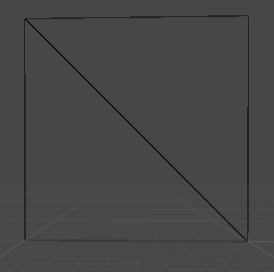
\includegraphics[width=0.35\linewidth]{Images/UnityQuadWireframe}
	\caption[Die Wireframeansicht des erstellten Meshes]{Die Wireframeansicht des erstellten Meshes im Unity Editor}
	\label{fig:unityquadwireframe}
\end{figure}

\subsection{Datenstrukturen f\"ur Meshes}
Wird zur Laufzeit eine Nachbarschaftsbeziehung abgefragt, zum Beispiel welche Faces oder Kanten an einem Punkt anliegen oder welche Endpunkte eine Edge hat, st\"o{\ss}t ein Indexed Mesh schnell an seine Grenzen. Diese Informationen lassen sich f\"ur ein solches Mesh \"uber eine ersch\"opfende Suche ermitteln, dessen Laufzeit von der gr\"o{\ss}e des Meshes abh\"angig ist. Um diese Probleme zu l\"osen gibt es unterschiedliche Datenstrukturen, die einzelne Komponenten eines Meshes direkt in eine Beziehung zueinander setzen.

\subsubsection{Triangle-Neighbor Structure}
Ein solcher Ansatzt ist die Triangle-Neighbor Structure (Dreiecks-Nachbar Struktur). Dabei erh\"alt jedes Dreieck eine Referenz auf jeden seiner Nachbarn und jeder Vertex speichert zus\"atzlich noch einen Pointer auf ein benachbartes Dreieck. Eine beispielhafte Implementierung sieht wie folgt aus \cite[S.269]{Shirley2010}:
\begin{lstlisting}
class Triangle 
{
	Triangle[3] Neighbours;
	Vertex[3] Vertices; 
}

class Vertex 
{
	// --- Vertex specific data
	Vector3 Point;
	Triangle Triangle;
}
\end{lstlisting}

Der Vorteil zu einem Indexed Mesh ist, dass nun nicht mehr jeder Punkt betrachtet werden muss, sondern mithilfe der Faces Aussagen \"uber das Mesh getroffen werden k\"onnen. Ein Problem, was beim traversieren des Meshes auftritt ist, dass nach jedem Schritt gepr\"uft werden muss, ob die n\"achste Face nicht gleichzeitig auch die letzte Face war. Damit dieses Problem nicht auftritt, kann von einem facebasierten Ansatz auf einen Edgebasierten umgestellt werden.

\subsubsection{Winged-Edge Mesh}
Eine edgebasierte Datenstruktur ist das Winged-Edge Mesh. Diese Datenstruktur besteht aus Edges, Faces und Vertices. Jede Face und jeder Vertex verweist auf eine anliegende Kante. Zudem besitzt jede Kante eine Referenz auf ihren Start- und Endpunkt (Head und Tail), die beiden anliegenden Faces sowie die beiden vorherigen und nachfolgenden Edges. Aus dieser Beschreibung ergibt sich eine solche Implementierung \cite[S.273]{Shirley2010}:

\begin{lstlisting}
class Edge
{
	Edge LeftPrevious, RightPrevious, LeftNext, RightNext;
	Vertex Head, Tail;
	Face Left, Right;
}

class Face 
{
	// --- Face specific data
	Edge Edge;
}

class Vertex 
{
	// --- Vertex specific data
	Vector3 Point;
	Edge Edge;
}
\end{lstlisting}

Die Vorteile \"uber der Triangle-Neighbor Structure sind, dass nicht nur Zugriffe zwischen Faces und Vertices konstant sind, sondern auch Abrufe von Kanten auf Dreiecke und Punkte vice versa sind in konstanter Zeit m\"oglich. Die Herausforderung beim Arbeiten mit einem Winged-Edge Mesh ist, dass immer drauf geachtet werden, aus welcher Richtung die aktuelle Edge kommt, um in der richtigen Richtung weiterzuarbeiten. Diese Unannehmlichkeit wird im Half-Edge Mesh gel\"ost.
\input{2_Grundlagen/Mesh}
\section{Half-Edge Mesh}
Um ein Traversieren eines Meshes, Abfragen der Nachbarschaftsbeziehungen der einzelnen Meshkomponenten und Operationen wie ,,Subdivisionen'' von Faces (Unterteilung der Faces in kleinere Dreiecke) so einfach wie m\"oglich zu machen, gibt es neben den oben genannten Ans\"atzen noch den Ansatz der Half-Edge Meshes. Ein solches Mesh besteht aus folgenden Komponenten:
\begin{itemize}
	\item eine Liste von Vertices
	\item eine Liste von Half-Edges
	\item eine Liste von Faces.
\end{itemize}

\begin{figure}[h]
	\centering
	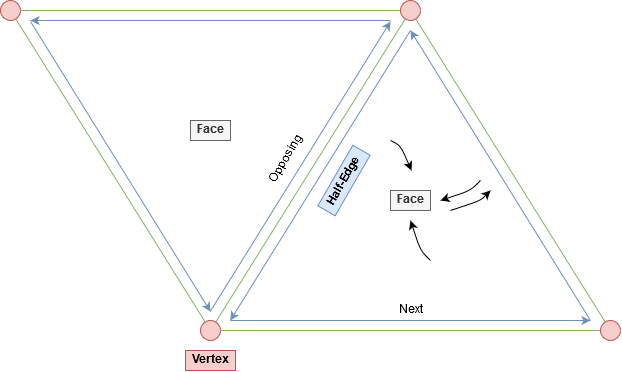
\includegraphics[width=0.7\linewidth]{Images/half-edge-mesh}
	\caption[Half-Edge-Mesh Schematik]{Die Elemente eines Half-Edge-Mesh.}
	\label{fig:half-edge-mesh}
\end{figure}

Im Gegensatz zu den Winged-Edge Meshes modellieren die Half-Edge Meshes eine Kante nicht explizit, sondern als Kombination aus zwei Half-Edges, die in jeweils entgegengesetzte Richtungen auf einen der Endpunkte der Kante zeigen, die Half-Edges sind gegen den Uhrzeigersinn orientiert. Durch die Aufteilung der Kanten kann jede Half-Edge genau einer Face zugeordnet werden und besitzt somit nicht mehr eine Referenz auf den linken und rechten Nachfolger, sondern einen nur noch einen Pointer auf die n\"achste Half-Edge der Face, wie in Abbildung \ref{fig:half-edge-mesh} gezeigt. Zudem Besitzt jede Half-Edge einen Verweis auf die zugeh\"orige Face sowie auf die Gegen\"uberliegende Half-Edge. Ein Verweis auf die Vorherige ist nicht n\"otig, da diese die \"ubern\"achste Kante ist. 

\subsection{Vergleich der Datenstrukturen}
Jede der vorgestellten Datenstrukturen kommt mit Vor- und Nachteilen. Die Entscheidung, welche von diesen verwendet wird, ist vom Use Case der Anwendung abh\"angig. Vergleichen kann man die Datenstrukturen in Sachen Speichernutzung und der Laufzeit von Nachbarschaftsabfragen. Bei der Speichernutzung wird ein allgemeines Mesh mit $n_v$ Vertices betrachtet, bei der Laufzeitanalyse wird zus\"atzlich mit $n_t$ die Anzahl der Dreiecke und mit $m_{ev}$ die Anzahl der Kanten pro Vertex dargestellt.

\begin{table}[ht]
	\caption{Vergleich der Datenstrukturen}
	\centering
		\begin{tabular}{|c|c|c|c|c|}
			\hline \rowcolor{gray}
		& Indexed Mesh & TNS & WEM & HEM \\ 
		\hline 
		Relativer Speicherbedarf & $36 \times n_v Byte$ & $116 \times n_v Byte$ & $228 \times n_v Byte$ & $228 \times n_v  Byte$ \\ 
		\hline 
		\multicolumn{5}{|c|}{Laufzeitanalyse der m\"oglichen Abfragen:} \\ 
		\hline 
		Edge $\rightarrow$ Vertices & N/A  & N/A & $\mathcal{O}(1)$ & $\mathcal{O}(1)$  \\ 
		\hline 
		Edge $\rightarrow$ Faces & N/A & N/A & $\mathcal{O}(1)$ & $\mathcal{O}(1)$ \\ 
		\hline 
		Edge $\rightarrow$ angrenzende Edges & N/A & N/A & $\mathcal{O}(n_{ev})$ & $\mathcal{O}(n_{ev})$ \\ 
		\hline 
		Vertex $\rightarrow$ Edges & $\mathcal{O}(n_t)$ & $\mathcal{O}(n_{ev})$ & $\mathcal{O}(n_{ev})$ & $\mathcal{O}(n_{ev})$ \\ 
		\hline 
		Vertex $\rightarrow$ Faces & $\mathcal{O}(n_t)$ & $\mathcal{O}(n_{ev})$ & $\mathcal{O}(n_{ev})$ & $\mathcal{O}(n_{ev})$ \\ 
		\hline 
		Face $\rightarrow$ Edges & $\mathcal{O}(1)$ & $\mathcal{O}(1)$ & $\mathcal{O}(1)$ & $\mathcal{O}(1)$ \\ 
		\hline 
		Face $\rightarrow$ Vertices & $\mathcal{O}(1)$ & $\mathcal{O}(1)$ & $\mathcal{O}(1)$ & $\mathcal{O}(1)$ \\ 
		\hline 
		Face $\rightarrow$ angrenzende Faces & $\mathcal{O}(n_t)$ & $\mathcal{O}(1)$ & $\mathcal{O}(1)$ & $\mathcal{O}(1)$ \\ 
		\hline 
	\end{tabular} 
	\label{Table:Comp}
\end{table}
Auff\"allig ist, dass der Speicherbedarf mit der Komplexit\"at des Netzes w\"achst, wodurch einzelne Abfragen beschleunigt oder erm\"oglicht werden. Zus\"atzlich f\"allt auf, dass das Winged-Edge Mesh gleich wie das Half-Edge Mesh abschneidet, allerdings bietet das Half-Edge Mesh in der Handhabung gro{\ss}e Erleichterungen, durch eine eindeutige Zuordnung von Half-Edge zu Face.

\subsection{Implementierung der Komponenten}
Die oben beschriebenen Komponenten sind im Folgenden in C\# implementiert, um das Half-Edge Mesh in Unity3D verwenden zu k\"onnen. 

\subsubsection{Klassenstruktur}
Aus den beschriebenen Elementen einer Half-Edge-Netzstruktur ergibt sich das in Abbildung \ref{fig:classdiagramhalfedgemesh} gezeigte Klassendiagramm. Der grundlegende Aufbau der einzelnen Klassen basiert dabei auf dem Plankton-Mesh \cite{Meshmash2017}. Jede Komponente besitzt eine eigene Listenklasse. Allerdings besitzen die einzelnen Komponenten im Plankton-Mesh keine direkte Referenz auf die benachbarten Komponenten, sondern einen Verweis auf den Index der Elemente in der jeweiligen Liste. So hat eine Half-Edge keine weitere Half-Edge als ,,Next'', sondern ein den jeweiligen Index der n\"achsten Kante.

\subsubsection{Die Vertex, HalfEdge und Face Klassen}
Die Klassen \textit{Vertex, HalfEdge} und \textit{Face} sind die Datenmodelle der oben beschriebenen Komponenten. Die Vertex-Klasse besitzt einen \textit{Vector3} Point, der die Position im Raum darstellt, eine \textit{HalfEdge}, die von diesem Punkt aus geht (Im Gegensatz zu \cite{Meshmash2017} wird hier eine Referenz gespeichert.) und der Index des Punktes, um die Arbeit mit dem Unity-Mesh zu erleichtern. Zudem kann ein \textit{PositionChangedEvent} abonniert werden, um Positions\"anderungen im Unity-Mesh direkt zu zeigen.
\\
Eine HalfEdge besitzt die oben erw\"ahnten Eingenschaften: den Punkt von dem sie ausgeht, die anliegende Face, die gegen\"uberliegende und n\"achste HalfEdge sowie den Index der HalfEdge. Wie auch der Index der Vertices, ist dieser Index f\"ur das Unity-Mesh wichtig.
\\
Die Face-Klasse besitzt eine Referenz auf eine anliegende HalfEdge und den Index der Face, diese wieder f\"ur die Arbeit mit dem Unity-Mesh.

\subsubsection{Listenklassen}
Objekte der Klassen \textit{Vertex, HalfEdge, Face} werden jeweils in einer Listenklasse gespeichert. Die Klassen \textit{VertexList, HalfEdgeList, FaceList} implementieren das \textit{IEnumerable}-Interface, um die Iteration \"uber die Elemente zu vereinfachen. Zudem beinhalten diese Klassen die Kernlogiken f\"ur die Komponenten. VertexList bietet die M\"oglichkeit, einen neuen Vertex hinzuzuf\"ugen oder einen zu entfernen, die HalfEdgeList verf\"ugt \"uber eine  \textit{CreateHalfEdge}-Methode, die wie folgt eine HalfEdge anlegt:

\begin{lstlisting}

public HalfEdge CreateHalfEdge(Vertex vertex, Face face, 
	HalfEdge next)
{
	HalfEdge halfEdge = new HalfEdge(vertex, face, next, Count);
	vertex.HalfEdge = halfEdge;
	// --- _halfEdges ist die zugrunde liegende Liste
	_halfEdges.Add(halfEdge);
	return halfEdge;
}

\end{lstlisting}

Und auch die FaceList besitzt eine Create-Methode, um eine Fl\"ache korrekt anlegen zu k\"onnen. Dabei wird die Referenz der Face auf die HalfEdge gesetzt und umgekehrt. Eine Weitere wichtige Methode ist die \textit{GetFaceCirculator}-Methode, die eine Liste aller HalfEdges, die an einer gegebenen Face anliegen, zur\"uck gibt:

\begin{lstlisting}
public List<HalfEdge> GetFaceCirculator(Face f)
{
	List<HalfEdge> result = new List<HalfEdge>();
	result.Add(f.HalfEdge);
	result.Add(f.HalfEdge.Previous);
	result.Add(f.HalfEdge.Previous.Previous);
	return result;
}
\end{lstlisting}

\begin{figure}[t]
	\centering
	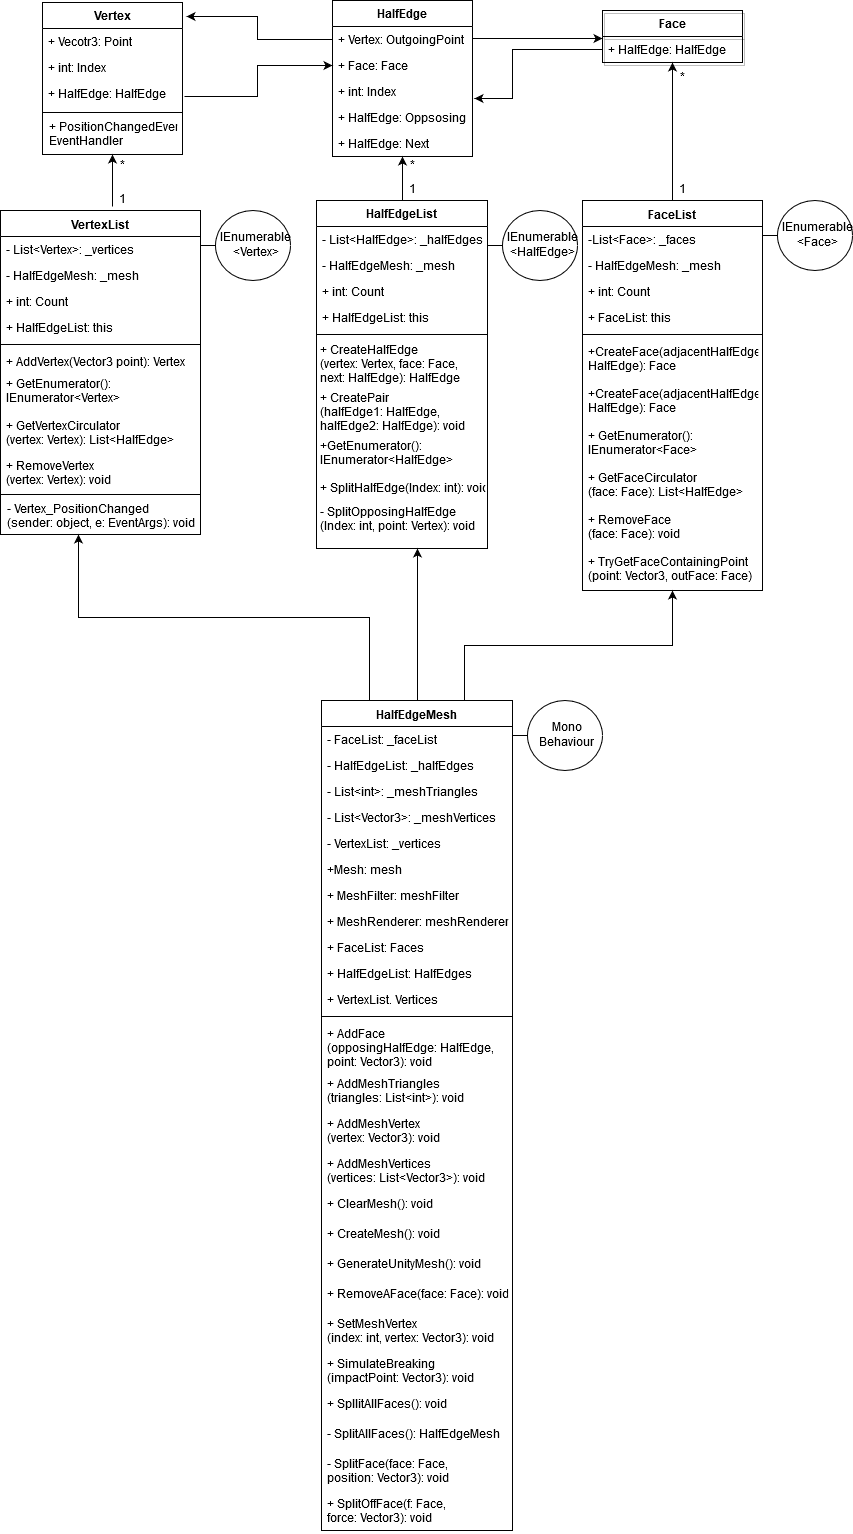
\includegraphics[width=0.7\linewidth]{Images/ClassDiagramHalfEdgeMesh}
	\caption[HalfEdgeMeshUMLDiagramm]{UML-Klassendiagramm des Half-Edge-Mesh Projekts}
	\label{fig:classdiagramhalfedgemesh}
\end{figure}


\subsection{Erstellen eines Half-Edge-Meshes}
Die Oben genannten Listenklassen werden von der \textit{HalfEdgeMesh}-Klasse verwendet, um aus der beschriebenen Half-Edge-Datenstruktur ein von Unity renderbares Mesh zu erstellen. 
\\
Um ein Dreieck, die einfachste m\"ogliche Netzstruktur zu erzeugen, kann die Methode \textit{CreateMesh} verwendet werden. Diese erstellt die drei Eckpunkte des Dreiecks, verbindet zwei mit einer neuen Half-Edge und erzeugt damit ein Face. Die Fl\"ache wird dann verwendet um die fehlenden Kanten mit Referenzen zu erzeugen und anschlie{\ss}end wird die Referenz der ersten Half-Edge auf die zweite gesetzt. Zum Schluss wird \textit{GenerateUnityMesh} aufgerufen um mit den angelegten Daten das UnityMesh zu generieren.
\begin{lstlisting}

public void CreateMesh(Vector3 va, Vector3 vb, Vector3 vc)
{
	Vertex a = Vertices.CreateVertex(va);
	Vertex b = Vertices.CreateVertex(vb);
	Vertex c = Vertices.CreateVertex(vc);

	HalfEdge heA = HalfEdges.CreateHalfEdge(a, null, null);
	Face face = Faces.CreateFace(heA);
	HalfEdge heB = HalfEdges.CreateHalfEdge(b, face, heA);
	HalfEdge heC = HalfEdges.CreateHalfEdge(c, face, heB);
	heA.Next = heC;

	GenerateUnityMesh();
}

\end{lstlisting}
Sollen beim erstellen des Netzes weitere Fl\"achen hinzugef\"ugt werden, ist es m\"oglich diese Methode zu erweitern oder weitere Faces mit \textit{AddFace} hinzuzuf\"ugen.

\subsubsection{GenerateUnityMesh}
Um aus den Daten des Half-Edge-Mesh ein f\"ur Unity brauchbares Mesh zu generieren, m\"ussen folgende Daten aus dem Half-Edge-Mesh entnommen werden: Die Position jedes Punktes, als Liste und ein Array mit der Reihenfolge, wie diese Punkte zu verbinden sind. Die Zusammenstellung dieser Daten passiert mit Hilfe von Linq. Hier der wichtigste Teil der \textit{GenerateUnityMesh}-Methode.
\begin{lstlisting}
	ClearMesh();
	// --- Add vertices
	List<Vertex> vertices = Vertices.Select(p => p.Point).ToList();

	// --- Add triangles
	foreach (Face face in Faces)
	{
		HalfEdge adjacentHalfEdges = Faces.GetFaceCirculator(face)
			.ToList();
		SetMeshTriangles(face.Index, adjacentHalfEdges
			.Select(p => p.OutgoingPoint.Index).ToList(), true);
	}

	AddMeshVertices(vertices);
	CommitMeshTriangles();
\end{lstlisting}
Da das Netz eines komplexen Modells sehr gro{\ss} werden kann, ist es f\"ur die Laufzeit von Vorteil, wenn bei lokalen \"Anderungen nicht das gesamte Netz neu generiert werden muss, wobei jedes Mal \"uber alle Punkte, Kanten und Fl\"achen iteriert werden muss. Stattdessen werden alle Punkte zus\"atzlich in einer Liste gespeichert, die beim bearbeiten des Netzes das UnityMesh aktualisiert. Werden dem Half-Edge-Mesh neue Punkte hinzugef\"ugt, k\"onnen diese mit den Methoden \textit{AddMeshVertex} und \textit{AddMeshVertices} erg\"anzt werden. Am Ende der Methode wird die aktualisierte Liste dem UnityMesh \"ubergeben. 

Auch die Triangles des UnityMeshes werden gecached. Da Manipulationen des Meshes in der Regel bedeuten, dass sich die Triangels relativ zu den drei Punkte einer Face ver\"andern, werden diese in dreier Tuplen in ein Dictionary geschrieben. Der Schl\"ussel ist dabei der Index der Face. Die Indexliste l\"asst sich mit \textit{SetMeshTriangles} bearbeiten. Dabei wird ein Eintrag an der Stelle des Faceindex hinzugef\"ugt, sofern er nicht vorhanden ist oder ver\"andert, falls ein Eintrag existiert. Wichtig ist dies zum Beispiel, wenn eine Face geteilt wird und ein Dreieckseintrag mit zwei von drei Punkten \"ubernommen wird. Als weiteren Parameter kann angegeben werden, ob eine Ver\"anderung Teil einer gr\"o{\ss}eren Transaktion war, um zu vermeiden, dass bei umfangreicheren Operationen, wie der Subdivision aller Faces, f\"ur jeden Methodenaufruf das Dictionary in eine Liste umzuwandeln und das Mesh erneut rendern zu m\"ussen. Wird diese Option verwendet, muss nach Abschluss der Transaktion \textit{CommitMeshTriangles} ausgef\"uhrt werden, um die \"Anderungen ins Mesh zu \"ubernehmen.

\subsubsection{GenerateHalfEdgeMesh}
Andersherum kann es genauso sinnvoll sein, ein bestehendes UnityMesh in ein Half-Edge Mesh umzuwandeln, um die Vorteile dieser nutzen zu k\"onnen. Die Logik dahinter befindet sich in der \textit{HalfEdgeMeshBuilder}-Klasse. Der Builder kann dem HalfEdgeMesh hinzugef\"ugt werden und besitzt eine Referenz auf das HalfEdgeMesh, um dieses bearbeiten zu k\"onnen. Um ein UnityMesh in ein HalfEdgeMesh zu \"uberf\"uhren, kann die \textit{BuildHalfEdgeMeshFromUnityMesh} verwendet werden. Diese Methode f\"ullt die drei Komponentenlisten anhand der Daten aus dem UnityMesh. 
Um dies zu erreichen gelten drei Grunds\"atze:
\begin{enumerate}
	\item F\"ur jeden Punkte gibt es einen Vertex
	\item F\"ur jeden Index gibt es eine HalfEdge, vom Punkt mit dem Index ausgehend
	\item Jeweils drei Indices bilden eine Face.
\end{enumerate}
\begin{lstlisting}
public void BuildHalfEdgeFromUnityMesh(Mesh mesh)
{
	List<Vector3> vertices = mesh.vertices;
	List<int> triangles = mesh.triangles;
	
	// --- Add vertices to HalfEdgeMesh
	int[] indexChanges = new int[vertices.Length];
	for (int i = 0; i < vertices.Length; i++)
	{
		Vector3 point = vertices[i];
		// --- CreateVertex checks if position is already saved 
		// --- and returns the first matching Vertex
		Vertex vertex = _mesh.Vertices.CreateVertex(point);
		
		// --- Saving the index change
		indexChanges[i] = vertex.Index;
	}
	
	// --- Change Vertex Index to first occurence
	if (indexChanges.Any())
	{
		for (int i = 0; i < triangles.Length; i++)
		{
			// --- change here!
			triangles[i] = indexChanges[triangles[i]];
		}
	}
	
	// --- For every three indices in triangles (= a face) add a face 
	// --- and three halfEdges
	for (int i = 0; i < triangles.Length - 3; i += 3)
	{
		Vertex point1 = _mesh.Vertices[triangles[i]];
		Vertex point2 = _mesh.Vertices[triangles[i + 1]];
		Vertex point3 = _mesh.Vertices[triangles[i + 2]];
		int[] indices = new[] {
			point1.Index, 
			point2.Index, 
			point3.Index 
		};
		List<HalfEdges> pairs = _mesh.HalfEdges
			.Where(p => indices.Contains(p.OutgoingPoint.Index)
			&& indices.Contains(p.EndPoint.Index));
	
		HalfEdge halfEdge1 = _mesh.HalfEdges
			.CreateHalfEdge(point1, null, null);
	
		Face face = _mesh.Faces.CreateFace(halfEdge1);
	
		HalfEdge halfEdge2 = _mesh.HalfEdges
			.CreateHalfEdge(point2, face, halfEdge1);
		HalfEdge halfEdge3 = _mesh.HalfEdges
			.CreateHalfEdge(point3, face, halfEdge2);
		halfEdge1.Next = halfEdge3;
	
		foreach (HalfEdge pair in pairs)
		{
			if (pair.OutgoingPoint.Index == halfEdge1.EndPoint.Index 
			&& pair.EndPoint.Index == halfEdge1.OutgoingPoint.Index)
				_mesh.HalfEdges.CreatePair(pair, halfEdge1);
			else if (pair.OutgoingPoint.Index == halfEdge2.EndPoint.Index 
			&& pair.EndPoint.Index == halfEdge2.OutgoingPoint.Index)
				_mesh.HalfEdges.CreatePair(pair, halfEdge2);
			else if (pair.OutgoingPoint.Index == halfEdge3.EndPoint.Index 
			&& pair.EndPoint.Index == halfEdge3.OutgoingPoint.Index)
				_mesh.HalfEdges.CreatePair(pair, halfEdge3);
		}
	}
}
\end{lstlisting}
Beim Erstellen des HalfEdgeMeshes muss beachtet werden, dass beim erzeugen eines Vertex mit \textit{\_mesh.Vertices.CreateVertex(point)} gepr\"uft wird, ob dieser Punkt bereits vorhanden ist, um redundante Daten zu vermeiden und ein zusammenh\"angendes Netz zu garantieren. Wenn in einem UnityMesh allerdings einen Punkt im \textit{vertices}-Array mehrfach vorkommt, verschieben sich nach dieser Stelle alle weiteren Indices. Somit muss zu beginn das UnityMesh ,,bereinigt'' werden. Beim Erstellen der Vertices werden etwaige Index\"anderungen gespeichert und f\"ur alle Indices gepr\"uft. Anschlie{\ss}end werden, wie beim erstellen des UnityMeshes auch, jeweils drei Indices gleichzeitig betrachtet.

Zu den Punkten hinter den Indices wird je eine HalfEdge erstellt und zu jeder Triplette wird eine Face erstellt, mit Referenz auf eine der HalfEdges. Zudem m\"ussen alle HalfEdges, die ein Paar mit einer aktuell betrachteten HalfEdge bilden, ermittelt werden. Daf\"ur werden alle HalfEdges gesucht, dessen eingehender und ausgehender Punkt in der Liste der aktuell betrachteten Punkte liegt: 
\begin{lstlisting}
List<HalfEdge> pairs = _mesh.HalfEdges
	.Where(p => indices.Contains(p.OutgoingPoint.Index)
	&& indices.Contains(p.EndPoint.Index));
\end{lstlisting}
\section{Operationen}
Nachdem ein Half-Edge Mesh prozedural erstellt wurde oder ein Unity Mesh umgewandelt wurde, k\"onnen auf ein Half-Edge Mesh einige Standardoperationen angewendet werden. Folgende Operationen werden im folgenden Kapitel erkl\"art und die Implementierung beschrieben:
\begin{itemize}
	\item das Teilen einer HalfEdge (Split HalfEdge),
	\item das Kollabieren einer Kante (Edge Collapse),
	\item das Aufteilen einer Face (Subdivision) und
	\item eine einfache 2D-Zerst\"orungssimulation (Simulate Breaking).
\end{itemize}

\subsection{Split Half-Edge}
Ziel der \textit{SplitHalfEdge}-Methode ist es, eine HalfEdge so zu teilen, dass das Ergebnis der Operation ein konformes Half-Edge Mesh ist, also dass jede Face immer noch aus drei Half-Edges besteht und dass jede Half-Edge maximal einen Partner besitzt. Um das Teilen durchzuf\"uhren, m\"ussen folgende Schritte durchgef\"uhrt werde, die in der Abbildung \ref{fig:splithalfedge} schematisch dargestellt sind:
\begin{enumerate}
	\item Bestimme die zu splittende HalfEdge.
	\item Erzeuge einen neuen Punkt, dort wo sich die HalfEdge aufteilt.
	\item Erzeuge drei neue HalfEdges und eine neue Face:
	\begin{itemize}
		\item Eine HalfEdge zum neuen Punkt, vom Ursprung der gesplitteten HalfEdge
		\item Eine HalfEdge als Nachfolger der ersten HalfEdge, mit dem neuen Punkt als Ursprung 
		\item Eine HalfEdge als Vorg\"anger der gesplitteten HalfEdge
	\end{itemize}
	\item Setze die Referenzen der HalfEdges neus
	\item F\"uhre Schritte 1-4 f\"ur die der gesplitteten HalfEdge gegen\"uberliegende HalfEdge ebenfalls aus
	\item Setze die Paare neu
\end{enumerate}

\begin{figure}[H]
	\centering
	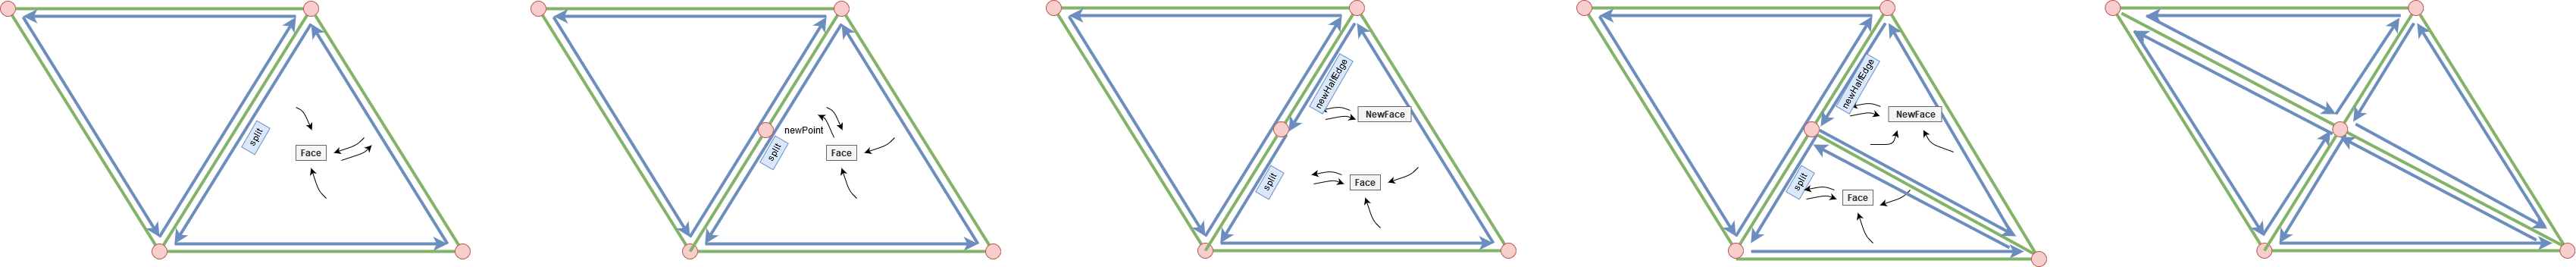
\includegraphics[width=1\linewidth]{Images/splitHalfEdge}
	\caption{Schematische Darstellung eines Edge splits. In Bild 1 ist die Ausgangssituation, Bild 2 zeigt Schritt 2, die Bilder 3 und 4 zeigen die Schritte 3 und 4 und Bild 5 zeigt das Ergebnis, nach den Schritten 5 und 6.}
	\label{fig:splithalfedge}
\end{figure}


Der beschriebene Algorithmus besitzt eine konstante Laufzeit, da die einzigen ,,komplexen'' Operationen auf der \textit{GetFaceCirculator}-Methode basieren, die immer die drei anliegenden HalfEdges einer Face zur\"uckgibt. Er ist im Folgenden implementiert:
\begin{lstlisting}
private bool _lock = false;
private HalfEdge _newHalfEdge, _split;

public void SplitHalfEdge(HalfEdge split, Vector3 splitPoint)
{
	// --- Schritt 1:
	split.Face.HalfEdge = split; // --- Set Reference of 
	// --- Face to split to know where the new face goes
	_split = split;

	// --- Schritt 2:
	Vertex newPoint = _mesh.Vertices.CreateVertex(splitPoint);

	// --- Schritt 3:
	HalfEdge newHalfEdge = _mesh.HalfEdges
	.CreateHalfEdge(split.OutgoingPoint, null, split);
	_newHalfEdge = newHalfEdge;
	Face newFace = _mesh.Faces.CreateFace(newHalfEdge);
	split.OutgoingPoint = newPoint;

	HalfEdge newHalfEdgeToSplit = _mesh.HalfEdges
	.CreateHalfEdge(split.Next.EndPoint, split.Face, split);
	HalfEdge newHalfEdgeFromNewHalfEdge = _mesh.HalfEdges
	.CreateHalfEdge(newPoint, newFace, split.Next.Next);
	_mesh.HalfEdges
	.CreatePair(newHalfEdgeToSplit, newHalfEdgeFromNewHalfEdge);

	// --- Schritt 4:
	newHalfEdge.Next = newHalfEdgeFromNewHalfEdge;
	newHalfEdgeFromNewHalfEdge.Next.Next = newHalfEdge;
	split.Next.Next = newHalfEdgeToSplit;

	// --- Aktualisiere das Unity Mesh
	_mesh.AddMeshVertex(newPoint.Point);
	
	_mesh.SetMeshTriangles(split.Face.Index,
	_mesh.Faces.GetFaceCirculator(split.Face)
	.Select(p => p.OutgoingPoint.Index)
	.ToList(), true);
	 
	_mesh.SetMeshTriangles(newFace.Index,
	_mesh.Faces.GetFaceCirculator(newFace)
	.Select(p => p.OutgoingPoint.Index)
	.ToList(), true);
	
	if (!_lock) // --- Blockiere nach dem ersten Aufruf,
				// --- um eine Endlosschleife zu vermeiden
	{
		// --- Schritt 5:
		if (split.Opposing != null) 
		{
			_lock = true;
			SplitHalfEdge(split.Opposing, splitPoint);
			// --- Schritt 6:
			_mesh.HalfEdges.CreatePair(_split, newHalfEdge);
			_mesh.HalfEdges.CreatePair(split, _newHalfEdge);
			_lock = false;
		}
	_mesh.CommitMeshTriangles();
	}
}
\end{lstlisting}
In wird die \textit{SplitHalfEdge}-Methode auf das erste Mesh in Abbildung \ref{fig:meshmash} angewendet, so ist das Mesh im zweite Bild das Ergebnis, wenn die Diagonale gesplittet wird und im Dritten, wenn die linke Kante unterhalb der Mitte geteilt wird. Das letzte Bild zeigt, dass der Teilungspunkt nicht zwingend auf der Kante liegen muss, da sich die Kanten entsprechend anpassen.
\begin{figure}[H]
	\centering
	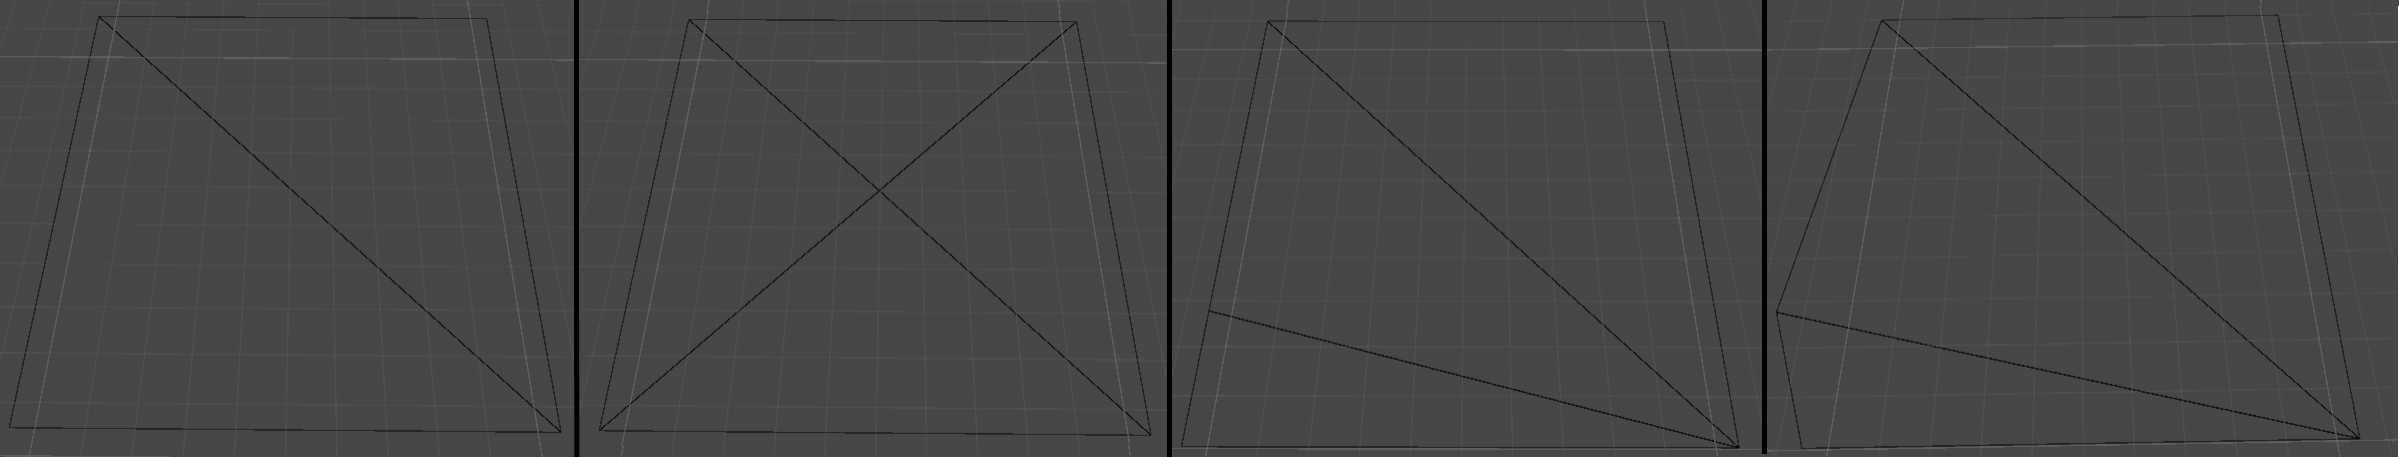
\includegraphics[width=1 \linewidth]{Images/meshmash}
	\caption{Bild 1 ist das Ausgangsmesh, welches in Bild 2 in der Mitte der Diagonale gesplittet wurde, in Bild 3 ein viertel auf dem Weg nach oben, auf der linken Seite und im 4. Bild eine Einheit links von der Kante}
	\label{fig:meshmash}
\end{figure}

\section{Vergleich zwischen Half-Edge Mesh und UnityMesh}
Nachdem die Funktionsweise der wichtigsten Operationen f\"ur ein Half-Edge Mesh im vorherigen Kapitel beschrieben wurden, werden diese im Folgenden mit vergleichbaren Operationen eines UnityMeshs verglichen.

Bei den Methoden \textit{SplitHalfEdge}, \textit{EdgeCollapse} und \textit{SplitFace} handelt es sich um Operationen auf dem Mesh, die lokale \"Anderungen verursachen. Da es einen direkten Zugriff auf die betroffenen Stellen gibt, mithilfe der Face- und Half-Edge-Listen muss nicht das gesamte Mesh nach den betroffenen stellen abgesucht werden. Zudem kann mittels der \textit{GetFaceCirculator}-Methode auf alle betroffenen Half-Edges in konstanter Zeit zugegriffen werden, da diese Methode immer die drei Half-Edges \"uber die Referenz der Face bestimmen kann. Insgesamt haben die \textit{SplitHalfEdge}- und \textit{SplitFace}-Methode also eine konstante Zeitkomplexit\"at, unabh\"angig von der gr\"o{\ss}e des Meshs.
Um allerdings das gleiche Resultat mit einem UnityMesh zu erhalten, muss zuerst mittels Brute-Force jeder Index der Eckpunkte der gesuchten Kante oder Face ermittelt werden, da diese nicht explizit dargestellt werden. Diese Suche nach allen Kanten mit den selben Eckpunkten k\"onnte wie folgt aussehen:
\begin{lstlisting}
List<int> findEdges(int a, int b)
{
	// --- All triangle indices
	int[] tris = _mesh.triangles;
	
	// --- The result contains every starting index of a matching triangle
	List<int> result = new List<int>();
	
	// --- for each pair of three
	for(int i = 0; i < tris.Length; i+=3)
	{
		int matches = 0; // --- count the matching indices
		if(tris[i] == a || tris[i] == b)
			matches++;
		if(tris[i+1] == a || tris[i+1] == b)
			matches++;
		if(tris[i+2] == a || tris[i+2] == b)
			matches++;
			
		// --- if there are two, consider this triangle index
		if(matches == 2) 
			result.Add(i);
	}
	return result;
}
\end{lstlisting}
Dieser beispielhafte Implementierungsvorschlag kann benutzt werden, um die betroffenen Faces f\"ur einen EdgeSplit zu finden, um die entsprechende Stelle f\"ur eine Subdivision zu finden, muss der dritte betroffene Punkt mitgegeben werden. Auff\"allig bei dieser Implementierung ist, dass es, im Gegensatz zum Half-Edge-Mesh abh\"angig von der gr\"o{\ss}e des Meshs ist, wodurch es bei dieser Implementierung mit gro{\ss}en Netzen zu Laufzeitproblemen kommen kann.

Auch die \textit{EdgeCollapse}-Methode verwendet die \textit{GetFaceCirculator}-Methode mit konstanter Laufzeit. Zus\"atzlich wird die \textit{GetVertexCirculator}-Methode verwendet, um die Half-Edges an den betroffenen Vertices zu finden. Theoretisch besitzt diese Methode eine konstante Laufzeit in Abh\"angigkeit von der Anzahl der Half-Edges, die den gefragten Vertex verwenden. Im Plankton-Mesh \cite{meshMash} wird folgende Implementierung verwendet:
\begin{lstlisting}
public IEnumerable<int> GetVertexCirculator(int halfedgeIndex)
{
	if (halfedgeIndex < 0 || halfedgeIndex > this.Count) { yield break; }
	int h = halfedgeIndex;
	int count = 0;
	do
	{
		yield return h;
		h = this[this.GetPairHalfedge(h)].NextHalfedge;
		if (h < 0) { throw new InvalidOperationException
		("Unset index, cannot continue."); }
		if (count++ > 999) { throw new InvalidOperationException
		("Runaway vertex circulator"); }
	}
	while (h != halfedgeIndex);
}
\end{lstlisting}
Allerdings funktioniert dieser Ansatz nur auf der zugrunde liegenden Annahme, dass das abgebildete Mesh vollst\"andig ist, es also keine Half-Edge gibt, die keinen Nachbarn hat. Aus diesem Grund wird eine andere Implementierung verwendet, da diese Eigenschaft f\"ur ein solches Netz nicht gegeben sein muss. Diese sieht wie folgt aus: 
\begin{lstlisting}
public List<HalfEdge> GetVertexCirculator(Vertex v)
{
	return _mesh.HalfEdges
	.Where(p => p.OutgoingPoint.Index == v.Index).ToList();
}
\end{lstlisting}
Durch diese Generalisierung wird allerdings die konstante Laufzeit durch eine Lineare ersetzt, wodurch die Laufzeiten des Half-Edge-Meshs und des UnityMeshs jeweils in lineare Abh\"angigkeit von der gr\"o{\ss}e des Netzes stehen. Allerdings kann, wie das Plankton-Mesh zeigt, die \textit{GetVertexCirculator}-Methode noch weiter optimiert werden. 

Alles in allem kann gesagt werden, dass ein Half-Edge-Mesh mit konstanten Laufzeiten f\"ur die wichtigsten Operationen besser geeignet ist f\"ur Echtzeitsimulationen mit dynamischen Meshs, die sich zur Laufzeit ver\"andern. Auch eignet sich ein Half-Edge-Mesh zur Bearbeitung eines Meshs, um den Detailgrad mithilfe der Subdivision zu erh\"ohen oder durch EdgeCollapse zu reduzieren. Allerdings kommen diese M\"oglichkeiten mit dem Nachteil, dass die Grundstruktur des Half-Edge-Mesh allein mehr als sechs mal so gro{\ss} ist, wie ein Indexed Mesh der selben Anzahl an Vertices. F\"ur statische Meshs eignet sich daher eher das UnityMesh und allgemein muss auf den einzelnen Anwendungsfall geachtet werden, um zu entscheiden, ob ein Half-Edge-Mesh oder ein Indexed Mesh verwendet werden soll.

\section{Ausblick}
Im Anschluss an diese Arbeit gibt es noch einige Features, um die diese Implementierung eines Half-Edge-Mesh erweitert werden kann. Zum Einen muss die \textit{GetVertexCirculator}-Methode optimiert werden, um eine konstante Zeitkomplexit\"at bei allen Grundoperationen zu erhalten, damit es in Echtzeitanwendungen verwendet werden kann. 

Des Weiteren ist ein Ziel, die 2D-Zerst\"orungssimulation zu erweitern, um diese in dreidimensionalen Simulationen verwenden zu k\"onnen. Dies kann geschehen, indem die Bruchpunkte nicht nur, wie bei der 2D-Simulation, auf der Oberfl\"ache, sondern auch innerhalb des Modells verteilt werden. Die erzeugten ,,Scherben'' werden um einen vierten Punkt erweitert, wodurch diese ein Tetraeder bilden und zu einem dreidimensionalen Splitter werden. 

In diesem Zuge sollte die Simulation auch die Kraft (force), die auf das Modell wirkt, betrachtet werden, um in unterschiedlichen Situationen realistischere Resultate zu erzielen.

Sollte der gew\"ahlte Ansatz nicht die gew\"unschten Effekte erzielen, kann eine andere Methode verwendet werden, um die Brucheffekte zu berechnen, zum Beispiel mithilfe von Voronoi-Diagrammen. 

Zum Schluss soll alles in einer Simulation zusammengef\"ugt werden, die als Demo dient, in der die Effekte gezeigt werden, um sie anschlie{\ss}end in Anwendungen, wie zum Beispiel Computerspielen verwenden zu k\"onnen.

\section{Rechnungen}
Um die Werte aus Tabelle \ref{Table:Comp} zu erhalten, m\"ussen folgende Annahmen getroffen werden: Bei der Speichernutzung wird ein allgemeines Mesh mit $n_v$ Vertices und $n_t$ Triangles betrachtet. Allgemein kann angenommen werden, dass ein Mesh ungef\"ahr doppelt so viele Eckpunkte wie Dreiecke hat, woraus sich $n_t \approx 2 * n_v$ ergibt. Zudem kann die Annahme get\"atigt werden, dass in C\# ein \textit{Vector3}, der aus drei \textit{floats} besteht eine Gr\"o{\ss}e von $3 * 32 Bit = 12 Byte$ hat, ein \textit{int} $4 Byte$ gro{\ss} ist und eine Referenz auf ein Objekt bei einer 64 Bit-Architektur $8 Byte$ ben\"otigt.
\subsection{Indexed Mesh}
$
n_v \times 12 Byte \mbox{(Vector3)} + 3 \times n_t \times 4 Byte \mbox{(Pro Dreieck gibt es 3 int Indices)} \\ \approx n_v \times 12 Byte + 6 n_v \times 4 Byte \\ 
\approx \underline{36 \times n_v Byte}
$

\subsection{Triangle-Neighbor Structure}
$
n_t \times (3 \times 8 Byte \mbox{(3 Referenzen auf Nachbardreiecke)} + 3 \times 8 Byte \mbox{(3 Referenzen auf Eckpunkte)}) + n_v \times (8 Byte \mbox{(Referenz auf ein anliegendes Dreieck)} + 12 Byte \mbox{(Vector3)}) 
\\\approx 2 \times n_v \times (24 Byte + 24 Byte) + n_v \times 20 Byte 
\\\approx 96 \times n_v Byte + 20 \times n_v Byte 
\\\approx \underline{116 \times n_v Byte}
$

\subsection{Winged-Edge Mesh}
$
n_v \times * (8 Byte \mbox{(Referenz von Vertex auf Edge)} + 12 Byte \mbox{(Vector3)}) + n_t \times 8 Byte \mbox{(Referenz von Face auf Edge)} + 1.5 n_t \mbox{(Jede Edge wird von zwei Faces verwendet)} \times (4 \times 8 Byte \mbox{Referenz der Kante auf andere Kanten} + 2 \times 8 Byte \mbox{(Referenz auf anliegende Faces)} + 2 \times 8 Byte \mbox{(Referenz auf Eckpunkte)}) 
\\\approx 20 \times n_v Byte + 2 \times n_v \times 8 Byte + 3 \times n_v \times 64 Byte
\\\approx 20 \times n_v Byte + 16 \times n_v Byte + 192 n_v Byte
\\\approx \underline{228 \times n_v Byte}
$

\subsection{Half-Edge Mesh}
$
n_v \times * (8 Byte \mbox{(Referenz von Vertex auf Edge)} + 12 Byte \mbox{(Vector3)}) + n_t \times 8 Byte \mbox{(Referenz von Face auf Edge)} + 3 \times n_t (4 \times 8 Byte \mbox{(Referenzen der HalfEdge auf den ausgehenden Punkt, die n\"achste und gegen\"uberliegende HalfEdge und die Face)})
\\\approx 20 \times n_v Byte + 2 \times n_v \times 8 Byte + 6 \times n_v \times 32 Byte
\\\approx \underline{228 \times n_v Byte}
$

%
%\section{Einleitung}
In der Computergrafik werden dreidimensionale Modelle als Polygonen-Netz (Polygonal Mesh) dargestellt, um diese auf einem zweidimensionalen Bildschirm darzustellen. Die Oberfl\"ache eines Modells wird dabei mit Hilfe von Polygonen angen\"ahert. H\"aufig werden daf\"ur Dreiecks-Netze (Triangle Mesh) verwendet, wobei die Fl\"achen mit Dreiecken nachmodelliert werden, siehe Abbildung \ref{fig:dolphintrianglemesh}. 
\\Ein solches Netz besteht aus den Eckpunkten der einzelnen Dreiecke, den Vertices. Diese werden durch Kanten (Edges) verbunden und bilden damit die Polygonalfl\"achen, auch Faces genannt. 

\begin{figure}[h]
	\centering
	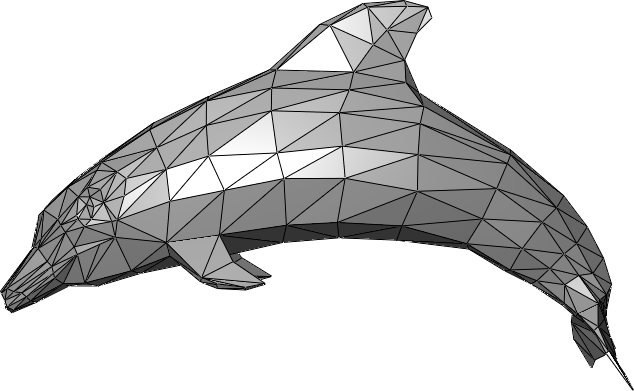
\includegraphics[width=0.7\linewidth]{Images/Dolphin_triangle_mesh}
	\caption[Beispiel eines Polygonen-Netzes]{Beispiel eines Dreiecks-Polygonen-Netz, von \cite{WikipediaDolphin1}}
	\label{fig:dolphintrianglemesh}
\end{figure}

\section{Unity}
Unity ist eine Spiele-Engine mit eingebauter Entwicklungsumgebung f\"ur 2D-, 3D- und VR-Spiele/-Simulationen. Die Engine kommt mit einem eigenen Editor, in welchem diverse Szenarien erstellt und bearbeitet werden k\"onnen. Des Weiteren unterst\"utzt Unity selbst programmierte Scripte auf der Grundlage von C\#.
\subsection{Meshes in Unity}
Unity bietet die M\"oglichkeit, mit Hilfe von selbstgeschriebenen Scripten eigene 3D-Modelle zur Laufzeit erstellen zu lassen. Daf\"ur stellt Unity ein eigenes Mesh-System zur Verf\"ugung, basierend auf Dreiecksnetzen, die \textit{UnityEngine.Mesh}-Klasse. Damit diese ein Mesh rendern kann, erwartet das Mesh ein \textit{UnityEngine.Vector3}-Array f\"ur die Vertices, wobei ein \textit{Vector3} einen Punkt im dreidimensionalen Raum darstellt und ein \textit{int}-Array, das die Reihenfolge der Vertices (\"uber die Indices der Vertices) f\"ur die Dreiecke festlegt.   
\\
Der folgende Code zeigt beispielhaft, wie ein Unity-Mesh erzeugt werden kann:
\begin{lstlisting}
public void CreateMesh()
{
	//--- Der Vollstaendigkeit halber vorhanden
	meshFilter = gameObject.GetComponent<MeshFilter>();
	if (meshFilter == null)
		meshFilter = gameObject.AddComponent<MeshFilter>();

	//--- vom MeshFilter zum Mesh
	mesh = meshFilter.sharedMesh;
	if (mesh == null)
		mesh = new Mesh { name = "Quad" };

	//--- MeshRenderer holen
	meshRenderer = this.gameObject.GetComponent<MeshRenderer>();
	if (meshRenderer == null)
		meshRenderer = gameObject.AddComponent<MeshRenderer>();

	//--- Mesh zusammenstellen
	//--- Vertices/Points
	var P0 = new Vector3(0, 0, 0);
	var P1 = new Vector3(0, 1, 0);
	var P2 = new Vector3(1, 0, 0);
	var P3 = new Vector3(1, 1, 0);
	
	var verticies = new List<Vector3> { P0, P1, P2, P3 };

	//--- Triangles
	var triangles = new List<int>();

	triangles.Add(0);
	triangles.Add(1);
	triangles.Add(2);
	triangles.Add(2);
	triangles.Add(1);
	triangles.Add(3);

	//--- Mesh befuellen
	mesh.Clear();
	//--- Vertices zuweisen
	mesh.vertices = verticies.ToArray();
	//--- Triangles zuweisen
	mesh.triangles = triangles.ToArray();
	//--- Mesh dem MeshFilter zuweisen
	meshFilter.sharedMesh = mesh;
}
\end{lstlisting}

Und liefert folgendes Ergebnis:
\begin{figure}[h]
	\centering
	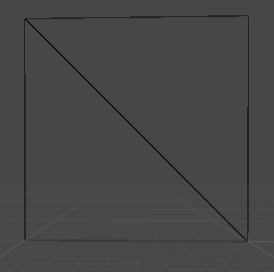
\includegraphics[width=0.35\linewidth]{Images/UnityQuadWireframe}
	\caption[Die Wireframeansicht des erstellten Meshes]{Die Wireframeansicht des erstellten Meshes im Unity Editor}
	\label{fig:unityquadwireframe}
\end{figure}

\subsection{Nachteile von Unity-Meshes}
Die Vorteile bei dieser Herangehensweise sind, dass die von Unity verwendeten Netze auch bei gr\"o{\ss}eren Netzen vergleichsweise wenig Speicherplatz ben\"otigen, da dieser Ansatz auf eine direkte Repr\"asentation von Faces und Edges verzichtet. Daraus ergeben sich einige Nachteile. Durch die fehlende Referenz auf die Polygonenfl\"achen sind Operationen auf Face-Ebene, wie eine Nachbarsuche, Abfragen auf alle Punkte Kanten oder die Unterteilung einzelner Polygonen in kleinere Einheiten (auch ,,Subdivision'' genannt), sehr Zeitintensiv, weshalb sich solche F\"alle nicht f\"ur Echtzeitanwendungen eignen. Des Weiteren stehen die Vertices im Unity-Mesh in keinem topographischen Zusammenhang, wodurch eine Iteration \"uber das gesamte Netz erschwert wird, um beispielsweise zusammenh\"angende Punkte zu bearbeiten.
	
%\section{Half-Edge-Mesh}
Um die oben genannten Problemstellungen zu l\"osen, gibt es andere Ans\"atze Polygonalnetze zu realisieren. Einer dieser L\"osungen ist das Konzept der Half-Edge-Meshes. Ein solches Mesh besteht aus folgenden Komponenten: 
\begin{itemize}
	\item eine Liste von Vertices
	\item eine Liste von Faces
	\item eine Liste von Half-Edges.
\end{itemize}

Die Vertices sind, wie im Unity-Mesh auch, die Eckpunkte der Polygonen. Die Vertices werden mithilfe von Half-Edges miteinander verbunden. 

\subsection{Vertex}
Ein Vertex ist ein Punkt im dreidimensionalen Raum und ist wie beim einfachen Mesh der Eckpunkt f\"ur die Polygonen. Neben einem \textit{Vector3} f\"ur die Position des Vertex wird eine Referenz auf eine ausgehende Half-Edge, sowie der Index des Vertex ben\"otigt.
\\
\begin{lstlisting}
public class Vertex
{
	public event EventHandler PositionChangedEvent;
	
	public Vertex(Vector3 point)
	{
		Point = point;
		Index = -1;
	}

	public Vertex(Vector3 point, int index)
	{
		Point = point;
		Index = index;
	}

	public Vertex(float x, float y, float z) : this(new Vector3(x, y, z))
	{ }

	public Vertex(float x, float y, float z, int index) : this(new Vector3(x, y, z), index)
	{ }

	/// <summary>
	/// The Index of the Vertex
	/// </summary>
	public int Index { get; set; }

	private Vector3 _point;
	/// <summary>
	/// The Point
	/// </summary>
	public Vector3 Point
	{
		get => _point;
		set
		{
			_point = value;
			PositionChangedEvent?.Invoke(this, EventArgs.Empty);
		}
	}

	/// <summary>
	/// The Outgoing HalfEdge
	/// </summary>
	public HalfEdge HalfEdge { get; set; }
}
\end{lstlisting}

\subsection{Face}
Ein Objekt der Klasse Face repr\"asentiert die Faces des Meshs, die \"uber die Vertices aufgespannt werden. Dabei besitzt eine Face nur die Referenz auf eine der anliegenden Half-Edges um das Traversieren und Bearbeiten des Netzes auf Face-Ebene zu erm\"oglichen. Die Face-Klasse ist wie folgt aufgebaut:
\begin{lstlisting}
public class Face
{
	public Face(HalfEdge halfEdge)
	{
		HalfEdge = halfEdge;
	}

	/// <summary>
	/// A bonding HalfEdge
	/// </summary>
	public HalfEdge HalfEdge { get; set; }
}
\end{lstlisting}

\subsection{Half-Edge}
Die Half-Edge Klasse ist die wichtigste Komponente f\"ur das Half-Edge-Mesh. Sie stellt alle Teile in Beziehung zueinander. Zu bemerken ist, dass ein Half-Edge-Mesh keine explizite Modellierung von Edges hat. Eine Edge wird implizit durch zwei Half-Edges abgebildet. Jede Half-Edge besitzt eine Referenz auf ihre gegen\"uberliegende Half-Edge, sowie auf die ihr Nachfolgende. Zudem referenziert jede Half-Edge den Vertex, aus dem sie hervorgeht und die Face, die sie einschlie{\ss}t. 
\begin{lstlisting}
public class HalfEdge
{
	public HalfEdge(Vertex outgoing, Face face, HalfEdge next)
	{
		OutgoingPoint = outgoing;
		Face = face;
		Next = next;
		Index = -1;
	}
	
	public HalfEdge(Vertex outgoing, Face face, HalfEdge next, int index)
	{
		OutgoingPoint = outgoing;
		Face = face;
		Next = next;
		Index = index;
	}
	
	public int Index { get; set; }
	
	/// <summary>
	/// The Vertex the HalfEdge comes from
	/// </summary>
	public Vertex OutgoingPoint { get; set; }
	
	/// <summary>
	/// The next HalfEdge, Counter Clockwise
	/// </summary>
	public HalfEdge Next { get; set; }
	
	/// <summary>
	/// The opposing HalfEdge
	/// </summary>
	public HalfEdge Opposing { get; set; }
	
	/// <summary>
	/// The face of the HalfEdge
	/// </summary>
	public Face Face { get; set; }
	
	/// <summary>
	/// Getter for the previous HalfEdge, for easier access 
	/// (this.Next.Next)
	/// </summary>
	public HalfEdge Previous => Next.Next;
	
	/// <summary>
	/// Getter for the EndPoint of this HalfEdge, for easier access (this.Next.OutgoingPoint)
	/// </summary>
	public Vertex EndPoint => Next.OutgoingPoint;
}
\end{lstlisting} 

%\section{Algorithmen}
\subsection{Subdivision von Faces}
\subsection{Teilen von HalfEdges}
\subsection{Breaking-Algorithmus}
\subsection{Smooting-Algorithmus}

\newpage

\bibliographystyle{alpha}
\bibliography{Literatur}

\end{document}